\section{Blokų grandinės technologija}

Blokų grandinė - tai vieno su kitu susijusių blokų grandinė, kurios blokuose saugomi
nekeičiami įrašai \cite{SatoshiNakamoto}. Šią technologiją galima apibūdinti kaip daugybę paskirstytų nekintamų skaitmeninių įrašų 
(angl. \textit{immutable distributed ledger}), tarpusavyje susietų taikant kriptografiją (blokų grandinės pavyzdys pateikiamas~\ref{fig:blockchain} paveiksle). Technologija geriausiai žinoma dėl jos panaudojimo Bitcoin kriptovaliutoje.
Šiame skyriuje apžvelgiami pagrindiniai blokų grandinės techniniai aspektai, savybės bei galimi skirtingi variantai.

\begin{figure}[H]
    \centering
    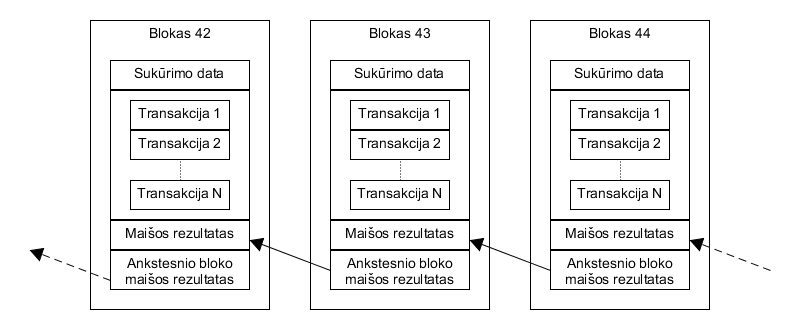
\includegraphics[scale=0.6]{img/blockchain}
    \caption{Supaprastintas blokų grandinės modelis}
    \label{fig:blockchain}
\end{figure}

\subsection{Nekintamumas}

Blokų grandinėje kiekvienas blokas yra sudarytas iš šių dalių:

\begin{enumerate}
    \item transakcijų. Kiekviena transakcija yra duomenys, kuriuos norima saugoti blokų grandinėje. Šie duomenys gali būti bet kokia vertinga informacija:
    finansinės transakcijos, programinis kodas, asmens duoti sutikimai (angl. \textit{consents}) ar kt. Kiekviena transakcija yra pasirašoma
    kūrėjo privačiu raktu. Vienas blokas gali turėti vieną arba daugiau transakcijų;
    \item bloko kriptografinės maišos funkcijos rezultato (angl. \textit{hash});
    \item ankstesnio bloko kriptografinės maišos funkcijos rezultato;
    \item bloko sukūrimo laiko. Blokai grandinėje saugomi chronologiškai;
    \item kitų metaduomenų (pvz. bloko eilės numerio).
\end{enumerate}

Kiekvieno bloko maišos funkcijos rezultatas priklauso nuo jo transakcijų, prieš tai buvusio bloko maišos rezultato ir bloko metaduomenų.
Jeigu betkurio bloko duomenys būtų pakeisti, tuomet maišos funkcija sugeneruotų kitokį maišos rezultatą ir būtų lengva patikrinti, kad
naujai perskaičiuotas maišos rezultatas nesutampa su bloke esančiu rezultatu. Taip pat, kadangi kiekvienas blokas
priklauso nuo prieš tai buvusio bloko, net ir pakeitus vieną iš pirmųjų blokų, pakeitimas būtų pastebimas pridedant naujus blokus ir būtų galima suprasti,
kad turima blokų grandinės versija yra nevalidi (žr.~\ref{fig:blockchainNotIntact} pav.). Tokiu būdu kiekvienas blokų grandinės blokas patvirtinta prieš tai
buvusio bloko integralumą, taip pasiekiant blokų grandinės nekintamumą (angl. \textit{immutability}),
nes perrašyti įrašus blokuose nepastebėtam labai sunku \cite{SatoshiNakamoto}.

\begin{figure}[H]
    \centering
    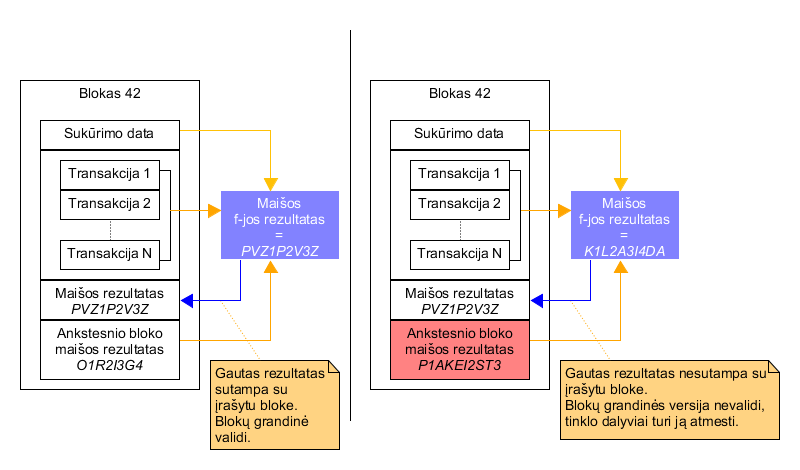
\includegraphics[scale=0.6]{img/blokchainNotIntact}
    \caption{Bloko grandinėje validavimas}
    \label{fig:blockchainNotIntact}
\end{figure}


\subsection{Decentralizacijos galimybės}

\subsection{Viešumo tipai}

\subsection{Konsensuso mechanizmas}